\section{Качество конечного многоклассового ответа}
\label{sec:multiclass_extended}
\subsection{Преимущество Ternary на естественном составе}
В отдельной общей семье M для CLINC150, TF3 $\to$ MiniLM,
natural, fit1000, квота20\%, MSE-настройка
\textbf{Ternary превосходит Hurdle одновременно по accuracy и macro-F1}.
Разница accuracy равна \NaturalAccuracyEffect{} п.п. с одновременным
интервалом $\NaturalAccuracyCI$ и $p=\NaturalAccuracyP$;
разница macro-F1 --- \NaturalFoneEffect{} п.п., интервал
$\NaturalFoneCI$, $p=\NaturalFoneP$.
Это пример прямого выигрыша одного gain-метода над другим
без искусственного изменения состава обучения.

\begin{table}[htbp]\centering\small
\caption{CLINC150, TF3 $\to$ MiniLM, natural, MSE-настройка:
многоклассовые метрики, средние по 20 обучениям.
Статистически установлен контраст Ternary--Hurdle;
таблица остальных кандидатов показывает полный контекст сравнения.}
\label{tab:natural_multiclass}
\begin{tabular}{lrrr}
\toprule
Метод & Accuracy, \% & Macro-P, \% & Macro-F1, \% \\
\midrule
Weak-error & 71{,}387 & 73{,}083 & 70{,}962 \\
Direct & 71{,}923 & 73{,}723 & 71{,}650 \\
Marginal & 71{,}373 & 73{,}073 & 70{,}947 \\
Events & 71{,}386 & 73{,}079 & 70{,}962 \\
Ternary & 71{,}603 & 73{,}321 & 71{,}212 \\
Joint & 71{,}577 & 73{,}275 & 71{,}176 \\
Hurdle & 71{,}310 & 73{,}011 & 70{,}878 \\
Soft-gain & 71{,}479 & 73{,}140 & 71{,}088 \\
Confidence & 71{,}911 & 73{,}812 & 71{,}788 \\
\bottomrule
\end{tabular}

\end{table}

\subsection{Какая информация добавляется к accuracy}
Метрики рассчитаны по истинным классам \emph{итогового ответа каскада}.
Восстановлены argmax-метки экспертов и решения маршрутизатора,
сохранены исходные tie-breaking и выбранные dev-параметры.
Всего пересчитаны 842\,760 строк скалярных метрик всех сохранённых
условий двух исследований. Для 42\,079 уникальных основных политик
классовые precision, recall и F1 независимо сверены со sklearn;
accuracy, спасения, вред и число вызовов воспроизвели прежние результаты.
На новых метриках роутеры не перенастраивались.

Для класса $c$ используются
\begin{equation}
P_c=\frac{TP_c}{TP_c+FP_c},\qquad
R_c=\frac{TP_c}{TP_c+FN_c},\qquad
F1_c=\frac{2TP_c}{2TP_c+FP_c+FN_c}.
\end{equation}
Нулевой знаменатель даёт 0; в усреднение входят все известные классы.
Macro-F1 --- среднее $F1_c$, а не гармоническое средних $P_c$ и $R_c$.
В single-label классификации без отказа micro-P/R/F1 и weighted-recall
совпадают с accuracy. Official test сбалансирован:
77 классов по 40 объектов в BANKING77 и 150 по 30 в CLINC150.
Поэтому здесь дополнительно macro-recall совпадает с accuracy,
а weighted-P/F1 --- с macro-P/F1. Новая агрегированная информация
содержится прежде всего в macro-precision и macro-F1.

Семья M включает все 36 попарных сравнений восьми обучаемых методов
и confidence в 33 конфигурациях: 21 BANKING77 и шесть CLINC150
при двух критериях настройки. Три метрики дают 3\,564 контраста;
bootstrap сохраняет support каждого класса. Найденное преимущество
Ternary относится к одному конкретному режиму и одной семье;
accuracy и macro-F1 оцениваются на тех же ответах и не являются
независимыми воспроизведениями.

\subsection{Разнонаправленные классовые эффекты при близких средних}
Другой описательный пример --- BANKING77, TF--IDF с одной меткой
на класс $\to$ tuned MiniLM. На natural Weak-error и Direct имеют
accuracy 42,742\% и 42,766\%, macro-precision 46,908\% и 47,446\%,
macro-F1 42,660\% и 42,827\%. Разница accuracy в 0,024 п.п.
соседствует с разницей macro-precision в 0,538 п.п.
Это возможно, потому что замена одной неправильной метки другой
меняет FP отдельных классов, сохраняя общую правильность.

Для класса \texttt{country\_support} F1 Weak-error и Direct
составляет 51,429\% и 39,530\%; для класса пополнения баланса
после чека или наличного депозита --- 40,910\% и 52,389\%.
Направления различий противоположны. Рисунок~\ref{fig:class_extended}
показывает перераспределение ошибок, скрытое близкой accuracy.
Пример выбран после просмотра среди 348 сравнений с разницей
средней accuracy не более 0,05 п.п., по максимальному абсолютному
расхождению macro-F1. Классы также отсортированы после просмотра;
при 40 объектах на класс это описательная диагностика,
а не проверка устойчивой классовой специализации.

\begin{figure}[htbp]\centering
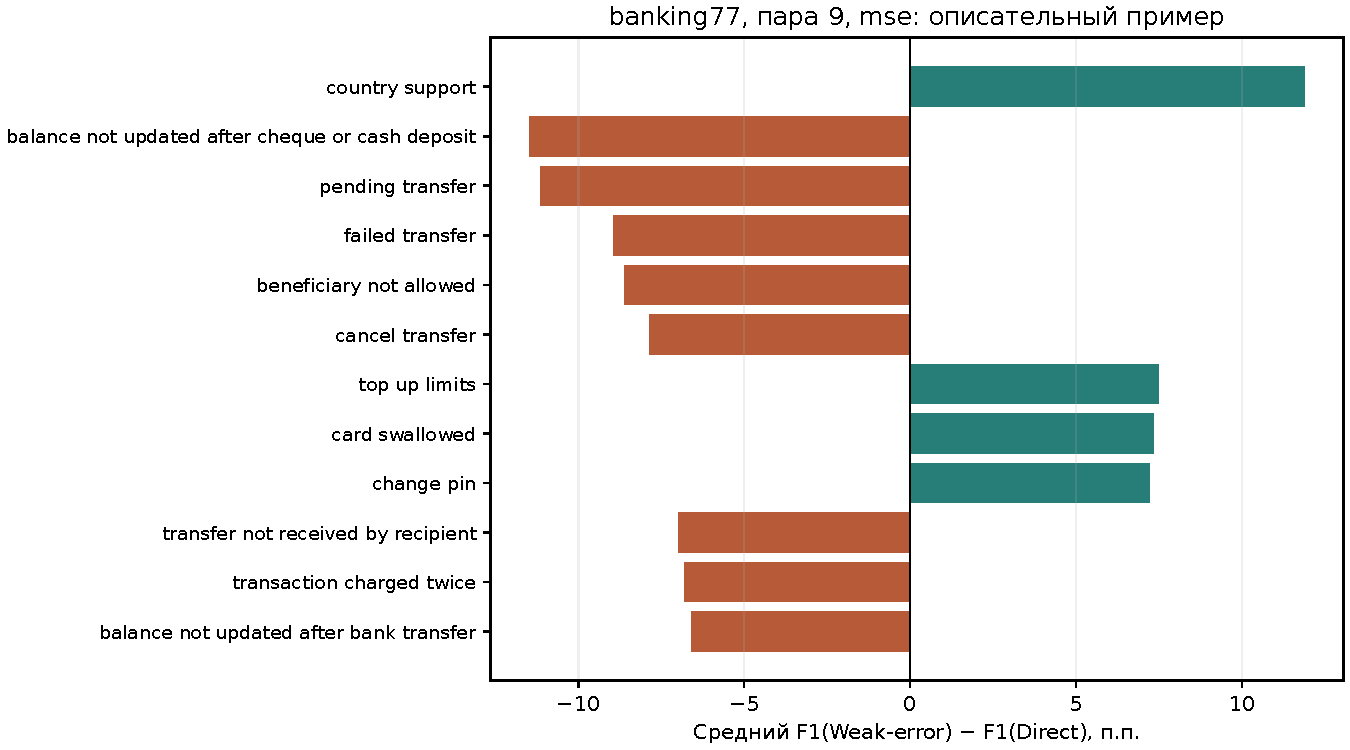
\includegraphics[width=.94\linewidth]{additions/figures/class_profile.pdf}
\caption{Описательный профиль Weak-error минус Direct,
BANKING77, TF--IDF с одной меткой на класс $\to$ tuned MiniLM.
Показаны 12 классов с наибольшим абсолютным расхождением
среднего F1; классовые p-values не вычислялись.}
\label{fig:class_extended}
\end{figure}
